%%%%%%%%%%%%%%%%%%%%%%%%%%%%%%%%%%%%%%%%%%%%%%%%%%%%%
%			HLAVIČKA								%
%%%%%%%%%%%%%%%%%%%%%%%%%%%%%%%%%%%%%%%%%%%%%%%%%%%%%
\documentclass[openany,12pt]{memoir}
\usepackage[utf8]{inputenc} 
\usepackage[czech]{babel}
\usepackage[T1]{fontenc}
\usepackage[top=1cm, bottom=2cm, left=2cm, right=2cm]{geometry}  % --> NASTAVENÍ OKRAJŮ
\usepackage{fancyhdr}
\usepackage{graphicx}
\usepackage{lmodern}
\usepackage{xwatermark}
\usepackage{xcolor}
\usepackage{changepage}
\chapterstyle{veelo}  %ALT BIANCHI, veelo
\usepackage{lettrine}
\usepackage{hyperref}



%%%%%% Package na zpěvník
\usepackage[full]{leadsheets}%http://mirrors.nic.cz/tex-archive/macros/latex/contrib/leadsheets/leadsheets_en.pdf   --> dokumentace	
\definesongtitletemplate{empty}{} 
\setchords{
format = \bfseries,   %tučné akordy
minor = {mi},% 
input-notation = {german},%
output-notation = {german}%
}
\definesongtitletemplate{empty}{} 

\newlength{\drop}
\newwatermark[pages=2-,color=red!50,angle=0,scale=2, xpos=0,ypos=0]{
\includegraphics[width=5cm]{obr/pozadi.jpg}} %--> dvojka na pozadí


%%%% Vlastní příkazy
\newcounter{Slokočet}   %Automatické číslování slok
\newcommand{\mezera}{\vspace*{0.5cm}}   %Horizontální odsazení slok
\newcommand{\stred}{5.2cm}   %%% Na zarovnání slok doprostřed, pozn. automatičtější zarovnávání na střed nejde
\newcommand{\refren}{\mezera \noindent \textbf{R:} } %refrén
\newcommand{\sloka}{\mezera \noindent \addtocounter{Slokočet}{1} \arabic{Slokočet}. } 	%sloka, která se automaticky čísluje
\newcommand{\ssloka}{\mezera \noindent}  % vlastní číslo sloky
\newcommand{\carka}{,\:}
\newcommand{\m}[1]{\color{white}{#1}}  %Pro akordy

\addto\captionsczech{\renewcommand{\contentsname}{Seznam koled}}

%%%%%%%%%%%%%%%%%%%%%%%%%%%%%%%%%%%%%%%%%%%%%%%%%%%%%%
%			NÁVOD									 %
%%%%%%%%%%%%%%%%%%%%%%%%%%%%%%%%%%%%%%%%%%%%%%%%%%%%%%
%1. Věci v hlavičce IGNOROVAT
%2. Píseň psát do prostoru mezi \begin{song} a \end{song}
%3. další řádek se značí dvěma odsazeníma (= dvakrát stisknout enter)
%4. \refren vždy na začátku refrenu a \sloka na začátek sloky (automaticky se čísluje)
%  \ = alt gr + q ; [/] = alt gr f/g ; {/} = alt gr + b/n; ^ = alt gr + 3 + mezera
%Cokoliv napíšete do ^{  } se bude brát jako akord
%když se toto bude dotýkat nějakého slova (nebude mezi tím a slovem mezera)
%tak se akordy zjeví nad slovem, ale pište to před slovo
%Když se to nedotýká slova, tak akord lítá ve vzduchu a vytiskne se větší mezera
%První možnost je asi preferovanější
%5. Akordy stačí psát jen do první sloky, když se nezmění -- kytaristi to zvládnou



%
%\usepackage{subfiles}
%</++>

\begin{document}\renewcommand{\abstractname}{\vspace{-\baselineskip}}
%Kompilovat dvakrát, aby se updatnula TOC
\pagestyle{empty}
\vspace*{4\baselineskip}
%%PŘEBAL
\moveright 12cm \vbox{
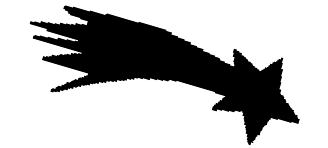
\includegraphics[width=5cm]{obr/comet.png}\\
}
\vspace*{4\baselineskip}
{\centering
\HUGE
\textbf{Vánoční zpěvník}\\
\Large
\begin{center}
\textbf{Pražské Dvojky}
\end{center}
\vspace*{3\baselineskip}
\begin{figure}[h]
\centering
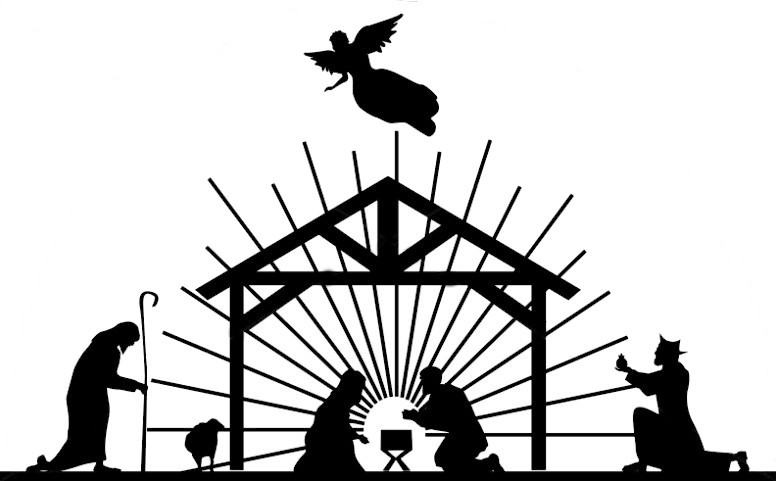
\includegraphics[scale=0.5]{obr/beth.jpg}
\end{figure}
}


\newpage

\vspace*{4\baselineskip}
\begin{abstract}
\large
\lettrine{D}{ržíte} v rukou speciální edici zpěvníku skautského oddílu Pražská Dvojka
s vánočními koledami. Za tímto zpěvníkem stojí spousta práce, avšak věříme, že se naše 
úsilí promění v úsměvy a dobrou náladu v pohodové atmosféře svátků Vánočních. Zpívání 
českých vánočních koled patří podle nás k duchu Vánoc neoddělitelně, a proto doufáme, že 
díky tomuto zpěvníku se Vám na tento zvyk alespoň jednou podaří najít ve vánočním shonu čas
ať už s námi, nebo v rodinném kruhu.\\
Zpěvník ke stažení a informace o našem oddíle najdete na stránkách www.dvojka.cz pod oddílem 
Pražská Dvojka.
\\\\\\\\\\
Veselé Vánoce přejí tvůrci zpěvníku:\\\\
Jindra \& Albert
\end{abstract}

\newpage
\setcounter{page}{1}
%\addtocontents{toc}{\protect\thispagestyle{empty}}
\tableofcontents* \thispagestyle{empty}\newpage
\newgeometry{top=1.5cm, bottom = 0cm, left = 2cm, right = 2cm}

\pagestyle{simple}

\addcontentsline{toc}{section}{Adeste Fideles}\begin{song}{title=\predtitle\centering Adeste Fideles \\\large John Francis Wade \vspace*{-0.3cm}}  %% sem se napíše jméno songu a autor
\begin{centerjustified}
\nejnejvetsi

\sloka 
	^{F{\color{white}aaa}}Adeste, ^{C}fidéles, ^{F{\color{white}aa}}laeti, ^{\,\,\,B\,\,\,\,F\,\,\,\,\,\,C}triumphántés

	^{Dmi\,G7}veníte, ^{C}veníte in ^{C\,\,\,\,\,\,G\,\,\,C}Béthlehem:

	^{F{\color{white}aaa}}Natum ^{\,\,Gmi\,F}vidéte ^{C\,\,\,F\,\,}Regem ^{Dmi\,G\,C\,\,\,\,\,\,}angelórum.
 

\refren
	^{F}Veníte ^{Gmi\,F{\color{white}aaa}}adorémus. ^{F}Veníte ^{B\,\,F\,C\,\,}adorémus.

	^{B}Veníte ^{{\color{white}aaaa}C\,Dmi}adorémus ^{F\,\,\,C\,\,F{\color{white}aa}}Dóminum.
 
 
\sloka
	En grege relícto, húmiles ad cunas
	
	vocáti pastóres appróperant:

	Et nos ovánti gradu festinémus.
 
 
\refren
 
 
\sloka
	Aetérni Paréntis splendórem aetérnum
	
	velátum sub carne vidébimus:
	
	Deum infántem, pannis involútum.
 
 
\refren
 
 
\sloka
	Pro nobis egénum et foeno cubántem:
	
	piis foveámus ampléxibus:
	
	Sic nos amántem quis non redamáret?
 
 
\refren


\end{centerjustified}

\setcounter{Slokočet}{0}
\end{song}


\newpage
\addcontentsline{toc}{section}{Bílé Vánoce}\begin{song}{title=\centering Bílé Vánoce \\\normalsize   \vspace*{-0.3cm}}  %% sem se napíše jméno songu a autor
\moveright 5.9cm \vbox{      %Varianta č. 1  ---> Jeden sloupec zarovnaný na střed	

\sloka 
	^{C}Já sním o ^{Dmi7}vánocích ^{F\#\,G7}bílých,

	^{F{\color{white}aaaa}}vánocích, ^{G7}jaké z dětství ^{C{\color{white}aaa}}znám, ^{Dmi7}

	^{G7{\color{white}aa}}zněly ^{\,\,C{\color{white}a}Cmaj7}zvonky ^{C7\,\,}saní

	a ^{F{\color{white}aaa}}každé ^{Fmi\,\,}přání v ten ^{C\,\,}den

	^{F{\color{white}aa}D7}splnilo se ^{Dmi7}nám. ^{G7}

\sloka
	Já sním o vánocích bílých,

	vánočním stromku zářícím,

	světla svíček, jmelí a sníh,

	tak byl krásný den o vánocích.



}
\setcounter{Slokočet}{0}
\end{song}

\newpage
\addcontentsline{toc}{section}{Byla cesta, byla ušlapaná}\begin{song}{title=\centering Byla cesta\carka byla ušlapaná \\\normalsize   \vspace*{-0.3cm}}  %% sem se napíše jméno songu a autor
\moveright 5.7cm \vbox{      %Varianta č. 1  ---> Jeden sloupec zarovnaný na střed	

\sloka 
	^{C}Byla cesta, ^{Fmi}byla ^{C}ušlapaná, 
	
	^{C}kdo ju ^{Fmi}šlapal, ^{C}kdo ju ^{Fmi}šlapal?

	^{B}Matka Krista ^{C}Pána.

\sloka
	Postřetla ju tam svatá Alžběta,

	kam ty kráčíš, kam ty kráčíš,
	
	sestřičko má milá?

\sloka
	Kráčím, sestro, kráčím do kostela,
	
	poslúchať mše, poslúchať mše,
	
	svatého nešpora.


\sloka
	Nechoď sestro, nechoď do kostela,
	
	povídajú, povídajú, 
	
	že porodíš syna.


\sloka
	Máš ho zrodit na ty slavné hody,
	
	když zamrznú, když zamrznú, 
	
	ve studénkách vody.

\sloka
	A co by to za novina byla,
	
	kdyby panna, kdyby panna
	
	syna porodila.

\sloka
	Porodila v ty vánoční hody,
	
	co zamrzly, co zamrzly
	
	všecky všady vody.

\sloka
	Není ptáčka, není křepelice,
	
	samé zimy, samé zimy,
	
	samé metelice.

\sloka
	Enem jedna voda nezamrzla,
	
	kde Maria, kde Maria
	
	pro vodu chodila,
	
	by Ježíšku, by Ježíšku
	
	kúpel udělala.



}
\setcounter{Slokočet}{0}
\end{song}

\newpage
\addcontentsline{toc}{section}{Dej Bůh štěstí tomu domu}\begin{song}{title=\predtitle\centering Dej Bůh štěstí tomu domu\\\large   \vspace*{-0.3cm}}  %% sem se napíše jméno songu a autor
\begin{centerjustified}
\nejnejvetsi

\sloka
	^{D\,\,}Dej ^{G\,\,}Bůh ^{D{\color{white}a}}štěstí tomu ^{A\,D{\color{white}a}}domu,

	^{D\,}my ^{G\,\,\,D{\color{white}aa}}zpíváme, víme ^{A\,D{\color{white}a}}komu,

	^{A7{\color{white}aaa}}malému ^{D}děťátku, ^{A7{\color{white}aa}}Kristu ^{D}Jezulátku,

	dnes ^{G}v ^{{\color{white}a}D}Betlémě ^{{\color{white}aa}Emi\,A7\,D}narozenému.

\sloka
	On rozdává štědrovníčky,

	jabka, hrušky a trojníčky,

	za naše zpívání, za koledování,

	dejž vám Pán Bůh své požehnání.



\end{centerjustified}
\setcounter{Slokočet}{0}
\end{song}

\newpage
\addcontentsline{toc}{section}{Chtíc, aby spal}\begin{song}{title=\centering Chtíc aby spal \\\normalsize   \vspace*{-0.3cm}}  %% sem se napíše jméno songu a autor
\moveright 5cm \vbox{      %Varianta č. 1  ---> Jeden sloupec zarovnaný na střed	

\sloka 
	^{D}Chtíc, ^{D7}aby ^{G}spal, tak ^{D7\,G}zpívala, ^{Ami\,D7\,G}synáčkovi,

	^{D}matka, ^{D7}jež ^{G\,D7\,G}ponocovala, ^{Ami\,D7\,G}miláčkovi:

	Spi, ^{D}nebes ^{G\,D}dítě ^{G\,Emi\,D}milostné, ^{Emi}Pán jsi ^{A7}a ^{D}Bůh,

	^{G}přeje ^{D}ti v ^{G\,D}lásce ^{C}celý ^{D}ráj, ^{Ami\,D7}pozemský ^{G}luh.

\sloka
	Dřímej, to matky žádost je, holubičko,
   
   	v tobě se duše raduje, ó, perličko!
   	
   	Nebesa chválu pějí tvou, slávu a čest,
	
	velebí tebe každý tvor, tisíce hvěz.

\sloka	
	Ó lilie, ó fialko, ó růže má,
	
	dřímej, má sladká útěcho, zahrádko má!
	
	Labuti má a loutno má, slavíčku můj,

	dřímej, má harfo líbezná, synáčku můj!

\sloka	
	Miláčku, spi a zmlkněte andělové,
   	
   	před Bohem se mnou klekněte, národové!
	
	Sestoupil v pravdě boží syn na naši zem,
	
	přinesl spásu, pokoj svůj národům všem.




}
\setcounter{Slokočet}{0}
\end{song}

\newpage
\addcontentsline{toc}{section}{I'm dreaming of home}\begin{song}{title=\centering I'm dreaming of home \\\normalsize Philippe Rombi \vspace*{-0.3cm}}  %% sem se napíše jméno songu a autor
\moveright 1cm \vbox{      %Varianta č. 1  ---> Jeden sloupec zarovnaný na střed
\begin{minipage}[t]{0.48\textwidth}\setlength{\parindent}{0.25cm}  %Varianta č. 2 --> Dva sloupce	

(Capo 1)


\sloka 
	I ^{D{\color{white}aa}}hear the mountain  ^{F#m{\color{white}a}}birds
	
	The ^{Emi{\color{white}aa}}sound of rivers ^{A{\color{white}aaa}}singing
	
	A ^{F#mi}song I've often  ^{Hmi{\color{white}a}}heard
	
	It ^{G{\color{white}aa}}flows ^{A{\color{white}aaaa}}through me ^{Hmi}now
	
	So ^{G{\color{white}aa}}clear ^{A{\color{white}a}}and so ^{Hmi{\color{white}a}}loud
	
	I ^{G{\color{white}aa}}stand  ^{A{\color{white}aaa}}where ^{Hmi}I am
	
	^{A{\color{white}a}}And ^{G}forever
	
	I'm ^{G{\color{white}aaa}A}dreaming of ^{D\,\,\,\,\,\,\,\,\,}home
	
	I ^{G{\color{white}aa}}feel ^{A}so ^{D}alone
	
	I'm ^{G{\color{white}aa}A{\color{white}a}}dreaming... of ^{D\,\,\,\,\,\,\,\,}home.

\sloka
	It's ^{D{\color{white}aa}}carried in the  ^{F#mi}air
	
	The ^{Emi\,\,\,}breeze of early ^{A\,\,\,\,\,\,\,\,\,\,}morning
	
	I  ^{F#mi}see the land so ^{Hmi}fair
	
	My ^{G{\color{white}aa}}heart  ^{A{\color{white}aa}}opens  ^{Hmi{\color{white}a}}wide
	
	There's ^{G{\color{white}a}A\,\,\,}sadness ^{Hmi}inside
	
	I ^{G{\color{white}aa}}stand  ^{A{\color{white}aaa}}where ^{Hmi}I am
	
	^{A{\color{white}a}}And ^{G}forever
	
	I'm ^{G{\color{white}aaa}A}dreaming of ^{D{\color{white}aa}}home
	
	I ^{G{\color{white}aa}}feel ^{A}so ^{D}alone
	
	I'm ^{G{\color{white}aa}A{\color{white}a}}dreaming... of ^{D{\color{white}a}}home.

\end{minipage}\begin{minipage}[t]{0.48\textwidth}\setlength{\parindent}{0.45cm}  % V případě varianty č.2 jde odsud text do pravé části
\vspace*{0.6cm}

\sloka	
	This ^{A}is no foreign  ^{C#mi}sky
	
	I ^{Hmi}see no foreign ^{E{\color{white}aa}}light
	
	But  ^{C#mi}far away am ^{F#mi}I
	
	From ^{D{\color{white}aa}}some ^{E{\color{white}aaaa}}peaceful  ^{F#mi{\color{white}a}}land
	
	I'm ^{D{\color{white}a}E{\color{white}a}}longing to ^{F#mi\,\,}stand
	
	A ^{D{\color{white}aa}}hand ^{E}in my  ^{F#mi}hand
	
	 ^{E{\color{white}a}}And ^{D}forever
	
	I'm ^{D{\color{white}aaa}E}dreaming of ^{A{\color{white}aa}}home
	
	I ^{D\,\,\,\,\,\,}feel ^{E}so ^{A}alone
	
	I'm ^{D\,\,\,\,\,\,\,E\,\,\,\,\,}dreaming... of ^{A{\color{white}a}}home.

\end{minipage}   %Součást druhé varianty
}
\setcounter{Slokočet}{0}
\end{song}

\newpage
\addcontentsline{toc}{section}{Já bych rád k Betlému}\begin{song}{title=\centering Já bych rád k Betlému \\\normalsize   \vspace*{-0.3cm}}  %% sem se napíše jméno songu a autor
\moveright 4cm \vbox{      %Varianta č. 1  ---> Jeden sloupec zarovnaný na střed	

\sloka 
	^{D}Já bych rád ^{Emi7}k Betlému, ^{D}k Ježíšku ^{A}malému.

	^{D}Mám doma ^{Emi7}křepeličku ^{D}a pěknou ^{Emi7\,A}žežuličku,

	^{D}ty mu ^{A7\,D}odvedu.

\sloka
	^{D}Bude ^{A}žežulička ^{D\,E7}vyrážet ^{A7}Ježíška. 

	^{D}U hlavičky jeho ^{Emi7\,A}sedávat, ^{D}líbezně mu bude ^{Emi7\,A}kukávat.

	^{D}Ku-kuku! Ku-kuku! Zdráv ^{G}budiž ^{A\,D}Ježíšku!

\sloka
	^{D}Bude ^{A}křepelička ^{D\,E7}vyrážet ^{A7}Ježíšku. 

	^{D}U hlavičky jeho ^{Emi7\,A\,D}sedávat, ^{D}\uv{pět peněz} mu bude ^{Emi7\,A}čítávat

	^{D}Pět peněz! Pět peněz! Ach, kýž ^{G}jsem v ^{A}nebi ^{D}dnes.



}
\setcounter{Slokočet}{0}
\end{song}

\newpage
\addcontentsline{toc}{section}{Jak jsi krásné neviňátko}\begin{song}{title=\predtitle\centering Jak jsi krásné neviňátko \\\large   \vspace*{-0.3cm}}  %% sem se napíše jméno songu a autor
\begin{centerjustified}
\nejnejvetsi

\sloka
	^{C\,}Jak jsi krásné ^{G{\color{white}aa}C{\color{white}aaa}}neviňátko, vprostřed bídy, ^{G7{\color{white}a}C{\color{white}aaa}}nebožátko,

	před Tebou ^{G{\color{white}aa}C{\color{white}a}}padáme, dary své ^{Dmi\,G7\,C}skládáme.

\sloka
	Já ti nesu dvě kožičky, by zahřály tvé údíčky;

	já zas trochu mlíčka, by kvetly tvá líčka.

\sloka
	Já ti nesu veselého beránka ze stáda svého;

	s ním si móžeš hráti, libě žertovati.

\sloka
	A co my ti, nuzní, dáme, darovati co nemáme;

	my ti zadudáme, písně zazpíváme.

\sloka
	Pastuškové mu dudajú, zvuky dud sa rozléhajú,

	slavně dudy dujú, všeci prozpévujú.

\sloka
	Měj se dobře, Jezulátko, přespanilé pacholátko!

	S tebú sa lúčíme, Bohu porúčíme.



\end{centerjustified}
\setcounter{Slokočet}{0}
\end{song}

\newpage
\addcontentsline{toc}{section}{Já malý přicházím}\begin{song}{title=\centering Já malý přicházím \\\normalsize   \vspace*{-0.3cm}}  %% sem se napíše jméno songu a autor
\moveright 4.5cm \vbox{      %Varianta č. 1  ---> Jeden sloupec zarovnaný na střed	

\sloka 
	^{D}Já malý přicházím ^{A{\color{white}aaaa}D\,\,}koledovat,
	
	co umím o Kristu ^{A7{\color{white}aaaa}D\,\,}prozpěvovat.
	
	Že se ^{A}narodil ^{D}v Betlémě ^{A}v chlévě, ^{D}chci ^{{\color{white}aaa}A7\,D}zvěstovat.

\sloka
	Chudý je, nahý je, trpí zimu,
	
	kdybych měl, co bych chtěl, dal bych jemu, 
	
	já malý žáček, plínku i fáček i peřinu.

\sloka
	Dost málo darujte, groš neb zlatý, 
	
	budete po smrti za to vzati
	
	do nebe jistě, pravím na místě, mezi svatý.


\sloka
	Jestli nic nedáte, nebroukejte 
	
	a na mé zpívání nefoukejte:
	
	až větší budu, líp zpívat budu, jen počkejte.


}
\setcounter{Slokočet}{0}
\end{song}

\newpage
\addcontentsline{toc}{section}{My tři králové}\begin{song}{title=\centering My tři králové \\\normalsize   \vspace*{-0.3cm}}  %% sem se napíše jméno songu a autor
\moveright 5.8cm \vbox{      %Varianta č. 1  ---> Jeden sloupec zarovnaný na střed	

\sloka 
	^{G}My tři ^{Emi\,Ami}králové ^{{\color{white}aa}D7}jdeme ^{G}k vám,

   ^{C{\color{white}aaa}}štěstí, ^{{\color{white}aa}Ami}zdraví, ^{D7}vinšujem ^{G{\color{white}a}}vám.

\sloka
	Štěstí, zdraví, dlouhá léta,
   	
   	my jsme k vám přisli z daleka.

\sloka	
	Z daleka je cesta naše,
   
   	do Betléma mysl naše.

\sloka
	Co ty, černej, stojíš vzadu,
   	
   	vystrkuješ na nás bradu.

\sloka
	A já černej vystupuju,
	
	a Nový rok vám vinšuju.

\sloka
	A my taky vystupujem
   	
   	a Nový rok vám vinšujem.



}
\setcounter{Slokočet}{0}
\end{song}

\newpage
\addcontentsline{toc}{section}{Narodil se Kristus Pán}\begin{song}{title=\predtitle\centering Narodil se Kristus Pán \\\large   \vspace*{-0.3cm}}  %% sem se napíše jméno songu a autor
\begin{centerjustified}
\nejnejvetsi

\sloka
	^{D{\color{white}aaaa}}Narodil ^{E7}se ^{A{\color{white}a}\,D{\color{white}a}}Kristus ^{A{\color{white}aa}}Pán, ^{E7\,A7\,E7}veselme ^{A}se,

	^{D}z růže ^{A{\color{white}aa}}kvítek ^{D{\color{white}aaa}}vykvet ^{A{\color{white}a}}nám, ^{D\,G\,D\,A7}radujme ^{D}se.

\refren
	^{D}Z života ^{{\color{white}aa}A\,D}čistého, z rodu ^{{\color{white}aaaaa}A\,D}královského,

	^{D7\,}nám, ^{G\,\,}nám ^{D\,G\,D\,A7}narodil ^{D}se.

\sloka
	Jenž prorokován jest, veselme se,

	ten na svět poslán jest, radujme se.

\refren

\sloka
	Člověčenství naše, veselme se,

	ráčil vzít Bůh na se, radujme se.


\refren

\sloka
	Goliáš oloupen, veselme se,

	člověk jest vykoupen, radujme se.


\refren


\end{centerjustified}
\setcounter{Slokočet}{0}
\end{song}
\newpage
\addcontentsline{toc}{section}{Nesem vám noviny}\begin{song}{title=\predtitle\centering Nesem vám noviny \\\large   \vspace*{-0.3cm}}  %% sem se napíše jméno songu a autor
\begin{centerjustified}
\nejvetsi

\sloka
	^{D{\color{white}aaa}}Nesem ^{G\,}vám ^{D{\color{white}a}G}noviny, ^{D\,{\color{white}aaaa}A\,D\,}poslouchejte,

	^{D\z G}z~betlémské ^{D{\color{white}aa}G\,}krajiny, ^{D{\color{white}aa}}pozor ^{A\,D\,}dejte.

	/: ^{D{\color{white}aaa}}Slyšte je pilně a ^{E7{\color{white}a}A7{\color{white}a}}neomylně :/, ^{D{\color{white}aa}A7\,D}rozjímejte. 

\sloka
	Syna porodila čistá Panna,

	v jesličky vložila Krista Pána.

	/: Jej ovinula a zavinula :/ plenčičkama.

\sloka
	K němužto andělé z nebe přišli,

	i také pastýři jsou se sešli.

	/: Jeho vítali, jeho chválili, :/ dary nesli.

\sloka
	Anděl Páně jim to sám přikázal

	když se jim na poušti všem ukázal,

	/: k Betlému jíti, neprodlévati :/ hned rozkázal.

\sloka
	Ejhle, při Kristovu narození

	stal se div veliký v okamžení,

	/: neboť noc tmavá se proměnila :/ v světlo denní.

\sloka
	Andělé v oblacích prozpěvují,

	narození Páně ohlašují,

	/: že jest narozen, v jeslích položen, :/ oznamují.

\sloka
	My také, křesťané, nemeškejme,

	k těm svatým jesličkám pospíchejme,

	/: Ježíše svého, Pána našeho :/ přivítejme.

\sloka
	Vítej nám, Ježíšku, z nebe daný,

	který se narodil z čisté Panny,

	/: pohlédni na nás a přijmi od nás :/ tyto dary.

\sloka
	Z nebe jsi sestoupil z pouhé lásky,

	krásné Jezulátko, kvítku rajský,

	/: jak jsi spanilý a ušlechtilý, :/ celý krásný.

\end{centerjustified}
\setcounter{Slokočet}{0}
\end{song}
\newpage
\addcontentsline{toc}{section}{Pásli ovce Valaši}\begin{song}{title=\centering Pásli ovce Valaši \\\normalsize   \vspace*{-0.3cm}}  %% sem se napíše jméno songu a autor
\moveright 6.5cm \vbox{      %Varianta č. 1  ---> Jeden sloupec zarovnaný na střed	

\sloka 
	^{C{\color{white}aa}}Pásli ^{G7}ovce ^{C{\color{white}aa}}Valaši,
	
	při ^{G7}betlémském ^{C{\color{white}a}}salaši.

\refren
	^{C{\color{white}aaa}}Hajdom hajdom ^{G7{\color{white}aa}\,C\,{\color{white}a}}tydlidom, 
	
	hajdom hajdom ^{G7{\color{white}aa}\,C\,{\color{white}a}}tydlidom.

\sloka
	Anděl se jim ukázal, 
	
	do Betléma jít kázal.	 

\refren

\sloka
	Jděte, jděte, pospěšte, 
	
	Ježíška tam najdete. 

\refren

\sloka
	On tam leží v jesličkách, 
	
	zavinutý v pleničkách. 
	
\refren

\sloka
	Anděl zpívá písničku, 

	pozdravuje matičku. 
	
\refren


\sloka
	Zdrávas, Panno Maria, 
	
	Matko Boží spanilá!. 
	
\refren

\sloka
	Maria se starala, 

	kde by plének nabrala. 

\refren

\sloka
	Utrhneme z růže květ, 
	
	obvineme celý svět. 
	
\refren


}
\setcounter{Slokočet}{0}
\end{song}

\newpage
\addcontentsline{toc}{section}{Půjdem spolu do Betléma}\begin{song}{title=\centering Půjdem spolu do Betléma \\\normalsize   \vspace*{-0.3cm}}  %% sem se napíše jméno songu a autor
\moveright 6cm \vbox{      %Varianta č. 1  ---> Jeden sloupec zarovnaný na střed	

\sloka 
	^{C}Půjdem spolu do Betléma,

	dujdaj, dujdaj, ^{D}dujdaj ^{G}dá!
	
\refren
	^{Dmi\,G7}Ježíšku, ^{C\,Ami}panáčku!

	^{Dmi}Já tě ^{G7}budu ^{C\,Ami}kolíbati,

	^{Dmi\,G7}Ježíšku, ^{C\,Ami}panáčku!

	^{Dmi}Já tě ^{G7}budu ^{C}kolíbat.

\sloka
	Začni, Kubo, na ty dudy:
	
	dujdaj, dujdaj, dujdaj dá! \dots

\refren

\sloka
	A ty, Janku, na píšťalku:
	
	dudli, tudli, dudli dá! \dots

\refren
   
\sloka
	A ty Mikši, na housličky:
	
	hudli, tydli, hudli dá! \dots

\refren

\sloka
	A ty, Vávro, na tu basu:
	
	rum, rum, rum, rum, ruma dá! \dots

\refren

}
\setcounter{Slokočet}{0}
\end{song}


\newpage
\addcontentsline{toc}{section}{Půlnoční}\begin{song}{title=\centering Půlnoční \\\normalsize   \vspace*{-0.3cm}}  %% sem se napíše jméno songu a autor
\moveright \stred \vbox{      %Varianta č. 1  ---> Jeden sloupec zarovnaný na střed	

\sloka 
	^{D{\color{white}aa}}Jedu domů po trati, jedu přes ^{{\color{white}aa}G}kopce, ^{A}

	^{D}za okny padá, padá sníh, budou ^{{\color{white}aaaa}G}Vánoce, ^{A}

	^{D{\color{white}aaaa}}chmury, trable, starosti, nechal jsem ve ^{{\color{white}aaa}G}městě, ^{A}

	už ^{D{\color{white}aaa}}slyším lidi na půlnoční zpívat v ^{{\color{white}aaaa}G}kostele, ^{A}

	^{\,D}aleluja, ^{{\color{white}a}Hmi}alelu -- -- ^{\,\,G}ja. ^{A} 

\sloka 
	Ježíš na kříži ztrápený občas se usměje

	na ty, co v zázrak uvěří, na ty co zpívají, 
	
	aleluja, aleluja. 
 
\refren
	Beránku ^{D\,\,}náš ^{A} na ^{{\color{white}aaaa}Hmi}nebesích, ^{G}

	stůj při ^{D\,\,}nás, ^{A} až přijde ^{C{\color{white}aa}}tma, 

	^{\,D}aleluja, ^{{\color{white}aa}Hmi}alelu -- -- ^{\,\,G}ja. ^{A} 
 

\sloka
	Stojím v prázdném kostele, hvězdy nade mnou, 
	
	z kříže zbyl jenom stín, ale přesto slyším, 
	
	aleluja, aleluja. 
	

\refren
	Beránku ^{D\,\,}náš ^{A} na ^{{\color{white}aaaa}Hmi}nebesích, ^{G}

	stůj při ^{D\,\,}nás, ^{A} až přijde ^{C{\color{white}aa}}tma, ^{G}

	beránku ^{D\,\,}náš ^{A} na ^{{\color{white}aaaa}Hmi}nebesích, ^{G}

	neopouštěj ^{D\,\,}nás, ^{A}až začnem se ^{C}bát, ^{Emi7}bát.  

	^{\,D}Aleluja, ^{{\color{white}aa}Hmi}alelu -- -- ^{\,\,G}ja, ^{A}
	
	^{\,D}aleluja, ^{{\color{white}aa}Hmi}alelu -- -- ^{\,\,G}ja, ^{A}
	
	^{\,\,D}aleluja. 

}
\setcounter{Slokočet}{0}
\end{song}

\newpage
\addcontentsline{toc}{section}{Purpura}\begin{song}{title=\centering Purpura \\\normalsize   \vspace*{-0.3cm}}  %% sem se napíše jméno songu a autor
\moveright 4cm \vbox{      %Varianta č. 1  ---> Jeden sloupec zarovnaný na střed	

\sloka 
	^{D}Tiše a ochotně purpura na ^{G}plotně voní, ^{D}stále voní,

	nikdo si nevšímá, jak život mění se v ^{A7}dým. ^{Emi\,A7}

\sloka
	^{D}Snad jenom v podkroví básníci bláhoví ^{G}pro ni slzy ^{D}roní,

	hrany jí odzvoní ^{A7}rampouchem ^{D\,G}křišťálovým. ^{D\,D7}

\sloka
	^{G}Slunce se vynoří, hned však se k pohoří ^{D}skloní, rychle skloní,

	a ^{Hmi}pak se ^{E}dostaví dlouhá a ^{A}pokojná ^{Dmi}noc. ^{Adim\,A7}

\sloka
	^{D}Tiše a ochotně purpura na plotně ^{G}voní, stále ^{D}voní,

	po ní k nám vklouzlo to ^{A7}tajemné kouzlo ^{D}vánoc. ^{G\,D}


}
\setcounter{Slokočet}{0}
\end{song}

\newpage
\addcontentsline{toc}{section}{Rolničky}\begin{song}{title=\centering Rolničky \\\normalsize   \vspace*{-0.3cm}}  %% sem se napíše jméno songu a autor
\moveright \stred \vbox{      %Varianta č. 1  ---> Jeden sloupec zarovnaný na střed	

\sloka 
	^{D{\color{white}aaa}}Sláva, už je sníh, jedem ^{F\#7}na ^{{\color{white}aaa}\,G}saních,

	^{Emi}kluci křičí, ^{D{\color{white}aaa}}zvonek ^{A}zní, jenom ^{A7}táta ^{D{\color{white}a}}ztich.

	^{D{\color{white}aaa}}Kouká na syna, uši ^{F\#7\,G}napíná ...

	^{Emi}Co to slyší ^{D}v ^{{\color{white}a}A}rolničkách? Na co ^{A7{\color{white}aaa}D{\color{white}aa}}vzpomíná?
    
\refren
	Rolničky, rolničky, kdopak ^{G}vám dal ^{D}hlas?

	^{G{\color{white}aaaaa}}Kašpárek ^{D{\color{white}aaaa}}maličký ^{E{\color{white}aa}}nebo děda ^{A7{\color{white}aa}}Mráz?

	^{D{\color{white}aaaaa}}Rolničky, rolničky, co to ^{G{\color{white}aaa}}zvoní v ^{D{\color{white}aa}}nich?

	^{G\,\,\,\,\,\,\,\,\,\,\,\,\,\,\,\,\,\,}Maminčiny ^{D\,\,\,\,\,\,\,\,\,\,\,\,\,}písničky, ^{Emi\,A7}vánoce a ^{D{\color{white}aa}}sníh.

\sloka
	Zvonky dětských let, rozezvoňte svět!

	Těm, co už jsou dospělí, ať je znova pět!
	
	Zvoňte zlehýnka, stačí chvilinka:
	
	Vzpomínka jak rolničky v srdci zacinká.
	
\sloka
	Jingle bells, jingle bells,
	
	Jingle all the way.
	
	Oh! what fun it is to ride
	
	in a one-horse open sleigh.
	

}
\setcounter{Slokočet}{0}
\end{song}

\newpage
\addcontentsline{toc}{section}{Rychle, bratři}\begin{song}{title=\centering Rychle\carka bratři \\\normalsize   \vspace*{-0.3cm}}  %% sem se napíše jméno songu a autor
\moveright 5.7cm \vbox{      %Varianta č. 1  ---> Jeden sloupec zarovnaný na střed	

\sloka 
	^{F{\color{white}aaaa}}Rychle, ^{C7{\color{white}aa}}bratři,	^{F{\color{white}aaa}}rychle ^{C7{\color{white}aaa}F\,\,\,\,}vstávejme, 
	
	do Betléma honem chvátejme, 
	
	^{F{\color{white}aa}}dary s sebou ^{C7{\color{white}aaaa}}vezměme

	a Ježíška pozdravme, 
	
	^{F{\color{white}aaa}}takto ^{C7{\color{white}aa}}jemu ^{F{\color{white}aaa}}zvučně ^{C7{\color{white}aaa}F\,\,\,\,}zahrajme!

	^{F{\color{white}aaaa}\,}Dudlaj, dudlaj, ^{Gmi{\color{white}aaaaa}}dudlajdá.
	
	^{F{\color{white}aaaa}\,}Dudlaj, dudlaj, ^{C7{\color{white}aaaa}}dudlajdá.

	^{F{\color{white}aaa}}takto ^{C7{\color{white}a}}jemu ^{F{\color{white}aaa}}zvučně ^{C7{\color{white}aaa}F\,\,\,\,}zahrajme!

\sloka
	Vítáme tě, Ježíšku malý, 
	
	pěkné my ti neseme dary, 
	
	dary tobě my dáme,
	
	které sami jen máme,
	
	k tomu tobě zvučně zahráme:

	Dudlaj, dudlaj, dudlajdá.
	
	Dudlaj, dudlaj, dudlajdá.

	K tomu tobě zvučně zahráme!


}
\setcounter{Slokočet}{0}
\end{song}

\newpage
\addcontentsline{toc}{section}{Štěstí, zdraví, pokoj svatý}\begin{song}{title=\centering Štěstí zdraví pokoj svatý \\\normalsize \vspace*{-0.3cm}}  %% sem se napíše jméno songu a autor
\moveright 4.5cm \vbox{      %Varianta č. 1  ---> Jeden sloupec zarovnaný na střed	

\sloka 
	^{C}Štěstí, zdraví, ^{G7}pokoj svatý ^{C\,G7}vinšujeme ^{C}vám,

	^{C}nejprv panu ^{G7}hospodáři ^{C}pak ^{G7}našim ^{C}dítkám.

	^{C}Zdaleka se béřeme, novinu vám neseme, 

	co jest se nám ^{G7}přihodilo v ^{C}městě ^{G7\,C}Betlémě.

\sloka
	Narodil se tam synáček, posílá mě k vám,
   	
   	byste mu koledy dali - však já mu ji dám.
   	
   	Chlebíčka nechce bráti, nakrmila ho máti,
   
   	radš tolárek neb dukátek máte poslati.

\sloka
	
	Pěkně prosím, odbuďte mě, nemám tu kdy stát,
   	
   	ještě musím do Betléma dítko kolíbat.
   
   	Dítko je to bohatý, v nebi vám to zaplatí,
   	
   	že se budete po smrti s ním radovati.

}
\setcounter{Slokočet}{0}
\end{song}

\newpage
\addcontentsline{toc}{section}{Tichá noc}\begin{song}{title=\centering Tichá noc \\\normalsize Franz Xaver Gruber \vspace*{-0.3cm}}  %% sem se napíše jméno songu a autor
\moveright 6cm \vbox{      %Varianta č. 1  ---> Jeden sloupec zarovnaný na střed	

\sloka 
	^{A{\color{white}aaa}}Tichá noc, svatá noc
	
	^{E{\color{white}a}}jala ^{E7}lid v ^{A{\color{white}aa}}blahý ^{A7}klid.
	
	^{D\,}Dvé jen srdcí tu ^{A}v Betlémě bdí,

	^{D{\color{white}aaa}}hvězdy při svitu ^{A}u jeslí dlí,
	
	^{E}v nichž malé ^{E7{\color{white}a}}děťátko ^{{\color{white}a}\,A\,A7}spí,
	
	^{A}v nichž malé ^{E}děťátko ^{A}spí.

\sloka
	Tichá noc, svatá noc!
	
	Co anděl vyprávěl,
	
	prišed s jasností v pastýřův stan,
	
	zní již z výsosti, z všech země stran:
	
	\uv{Vám je dnes spasitel dán;
	
	přišel Kristus pán!}


\sloka	
	Tichá noc, svatá noc!
	
	Ježíšku na líčku
	
	boží láska si s usměvem hrá,
	
	zpod zlaté řasy k nám vyzírá,
	
	že nám až srdečko plá,
	
	vstříc mu vděčně plá.

}
\setcounter{Slokočet}{0}
\end{song}

\newpage
\addcontentsline{toc}{section}{Vánoce, Vánoce přicházejí}\begin{song}{title=\centering Vánoce\carka Vánoce přicházejí \\\normalsize   \vspace*{-0.3cm}}  %% sem se napíše jméno songu a autor
\moveright 4cm \vbox{      %Varianta č. 1  ---> Jeden sloupec zarovnaný na střed	

\refren
	^{C{\color{white}aaaa}}Vánoce, vánoce ^{G7{\color{white}aaaaa}}přicházejí, 

	zpívejme ^{{\color{white}aaa}C}přátelé,

	po roce vánoce, vánoce ^{G7{\color{white}aaaaa}}přicházejí,

	šťastné a ^{{\color{white}aaa}C}veselé.

\sloka
	^{G7}Proč jen děda říct si nedá, ^{D7{\color{white}a}}tluče o stůl v ^{G{\color{white}aaaa}}předsíni

	a pak, běda, marně hledá ^{D7{\color{white}a}}kapra pod ^{{\color{white}aa}G}skříní.

	Naše teta peče léta ^{D7}na vánoce ^{G{\color{white}aaaaa}}vánočku,

	nereptáme, aspoň máme ^{D7{\color{white}a}}něco pro ^{{\color{white}aa}G}kočku.  ^{G7}Jó!
      
\refren
   
\sloka
	Bez prskavek, tvrdil Slávek, na Štědrý den nelze být

	a pak táta s minimaxem zavlažoval byt.

	Tyhle ryby neměly by maso míti samou kost,
	
	říká táta vždy, když chvátá na pohotovost.


\refren

\sloka
	Jednou v roce na vánoce strejda housle popadne,

	jeho vinou se z nich linou tóny záhadné.

	Strejdu vida děda přidá \uv{Neseme vám noviny}

	čímž prakticky zničí vždycky večer rodinný.


\refren

\sloka
	A když sní se, co je v míse, televizor pustíme,
	
	v jizbě dusné všechno usne v blaženosti své.
	
	Mně se taky klíží zraky, bylo toho trochu moc,
	
	máme na rok na klid nárok, zas až do Vánoc.

\refren



}
\setcounter{Slokočet}{0}
\end{song}

\newpage
\addcontentsline{toc}{section}{Veselé vánoční hody}\begin{song}{title=\predtitle\centering Veselé Vánoční hody \\\large   \vspace*{-0.3cm}}  %% sem se napíše jméno songu a autor
\begin{centerjustified}
\nejnejvetsi

\sloka
	^{D}Veselé ^{{\color{white}aa}\,\,G\,D}vánoční ^{A7\,D}hody, zpívejte ^{{\color{white}aa}G}dítky ^{D\,A7\,D}koledy,

	o tom, co se ^{A{\color{white}aaaa}}vskutku stalo, ^{D}že se lidem ^{A{\color{white}aaaa}}narodilo,

	^{D\,A7\,D}děťátko.

\sloka
	On je světa Spasitelem, Slovo učiněné tělem,

	Syn Boží a syn člověka, na nějž tvorstvo věky čeká,

	děťátko.

\sloka
	Jehož Maria počala, v Betlémě ho porodila,

	položila do jesliček, zavinula do plenčiček,

	děťátko.

\sloka
	Vůl a oslík nad ním stáli a svým dechem zahřívali

	chudé lidské nemluvňátko, slavné Boží pacholátko,

	děťátko.

\sloka
	Potmě leží, nemá svíčičky, na nebi svítí mu hvězdičky.

	Ty, jenž všechen oděv dáváš, samo's nahé a nic nemáš,

	děťátko.

\sloka
	Přišli chudí pastouškové, zpívají ti chvály nové:

	Vítej nám, nebeský Králi, Tebeť jsme zdávna žádali,

	děťátko.

\end{centerjustified}
\setcounter{Slokočet}{0}
\end{song}

\newpage
\addcontentsline{toc}{section}{Z jedné strany chvojka}\begin{song}{title=\predtitle\centering Z jedné strany chvojka \\\large   \vspace*{-0.3cm}}  %% sem se napíše jméno songu a autor
\begin{centerjustified}
\nejnejvetsi

\sloka 
	^{D}Z jedné strany chvojka, ^{G}z druhé ^{D}borověnka.

	/: ^{G}Pásli ovce ^{D{\color{white}aaaaaaaa}}pastuškové, ^{A7{\color{white}a}}jedli kaši ^{\,D}z hrnka. :/

\sloka
	Přiletěl k nim anděl, aby jim pověděl 
	
	/: že se Kristus Pán narodil, aby každý věděl.:/

\sloka
	A my hoši malí, rádi by chom brali.
	
	/: Koledičku na ručičku, kdybyste nám dali. :/
	
\sloka
	Jestli nic nedáte, potom uhlídáte.
	
	/: Všechny hrnce vám roztlučem, co v mísníku máte. :/


\sloka
	A pokličky k tomu, pak utečem domů.
	
	/: Protože jste nechtěli dát koledy nikomu. :/

\end{centerjustified}
\setcounter{Slokočet}{0}
\end{song}

\newpage




%Nejsem si jistý, jestli chceme mít tohle na poslední straně
\newgeometry{top=1cm, bottom = 1cm, left = 1cm, right = 1cm}
\thispagestyle{empty}
\begin{figure}[h]
\centering
\includegraphics[height=\textheight]{../../Akordy/Akordymale.pdf}
\end{figure}



\end{document}

